\documentclass{beamer}
\usepackage[utf8]{inputenc}
\usepackage{amssymb}
\usepackage{xcolor}

\title[Nelder-Mead on the Rhology Problem]{Chapter 5 Project: Apply Nelder-Mead to the Rheology Problem}
\author[Matthew, Tyler, and Sarah]{Matthew Saurette, Tyler Weames, and Sarah Wyse}
\institute[Math 462]{Math 462\\ University of British Columbia - Okanagan}
\date{December 2020}
\usetheme{Madrid}
\usecolortheme{seahorse} 
\useinnertheme{rounded}

\begin{document}
\maketitle

\begin{frame}{Nelder-Mead Algorithm}
    \centering
    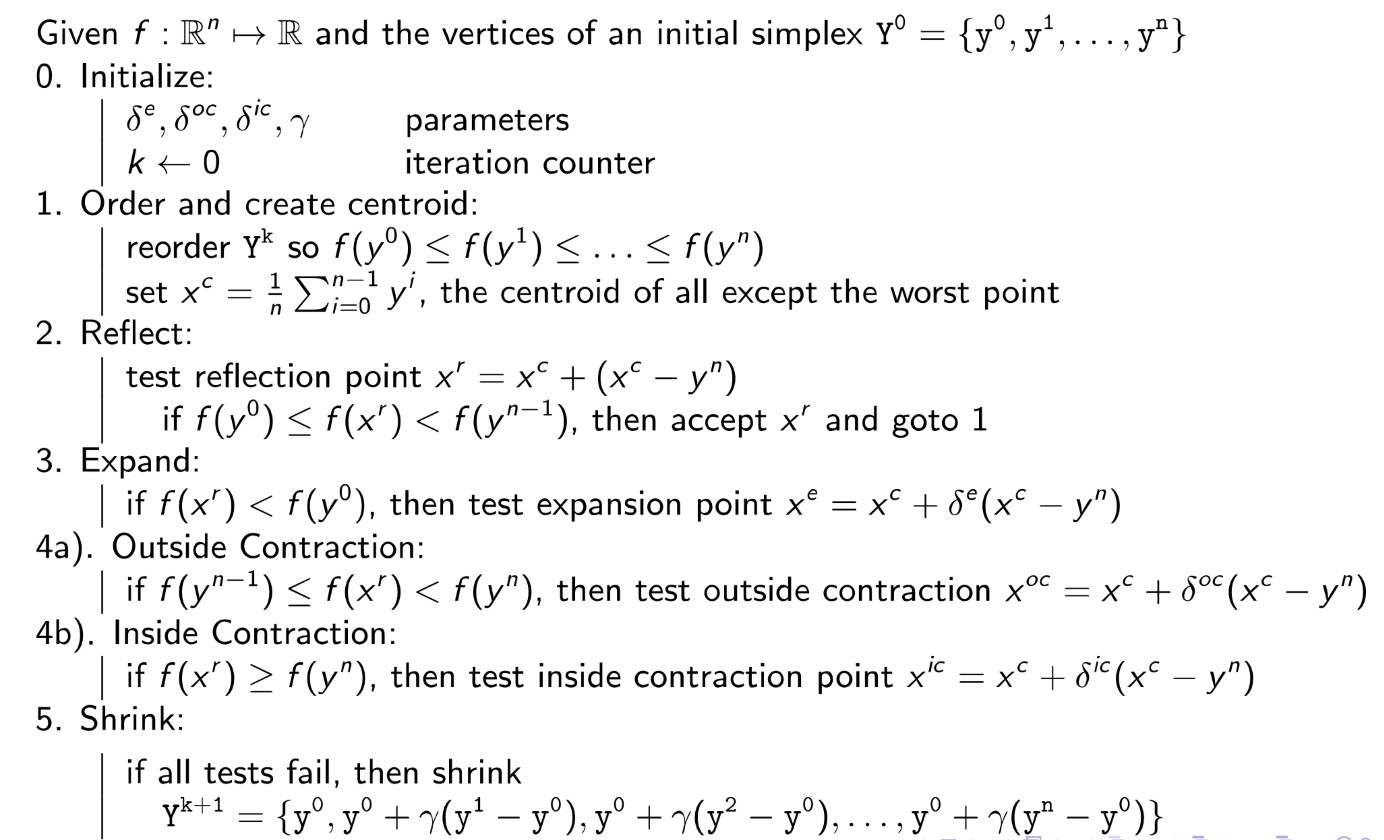
\includegraphics[width=0.95\linewidth]{NMAlgorithm}\\
    \tiny
	\hfill Algorithm from lecture slides    
\end{frame}

\begin{frame}{0. Initialize}
	\centering
	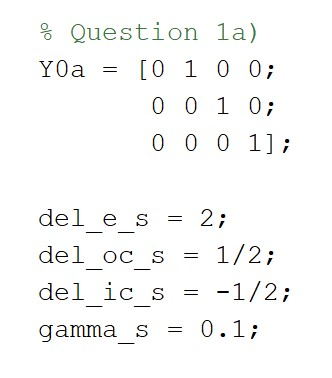
\includegraphics[width=0.45\linewidth]{Initialize}
	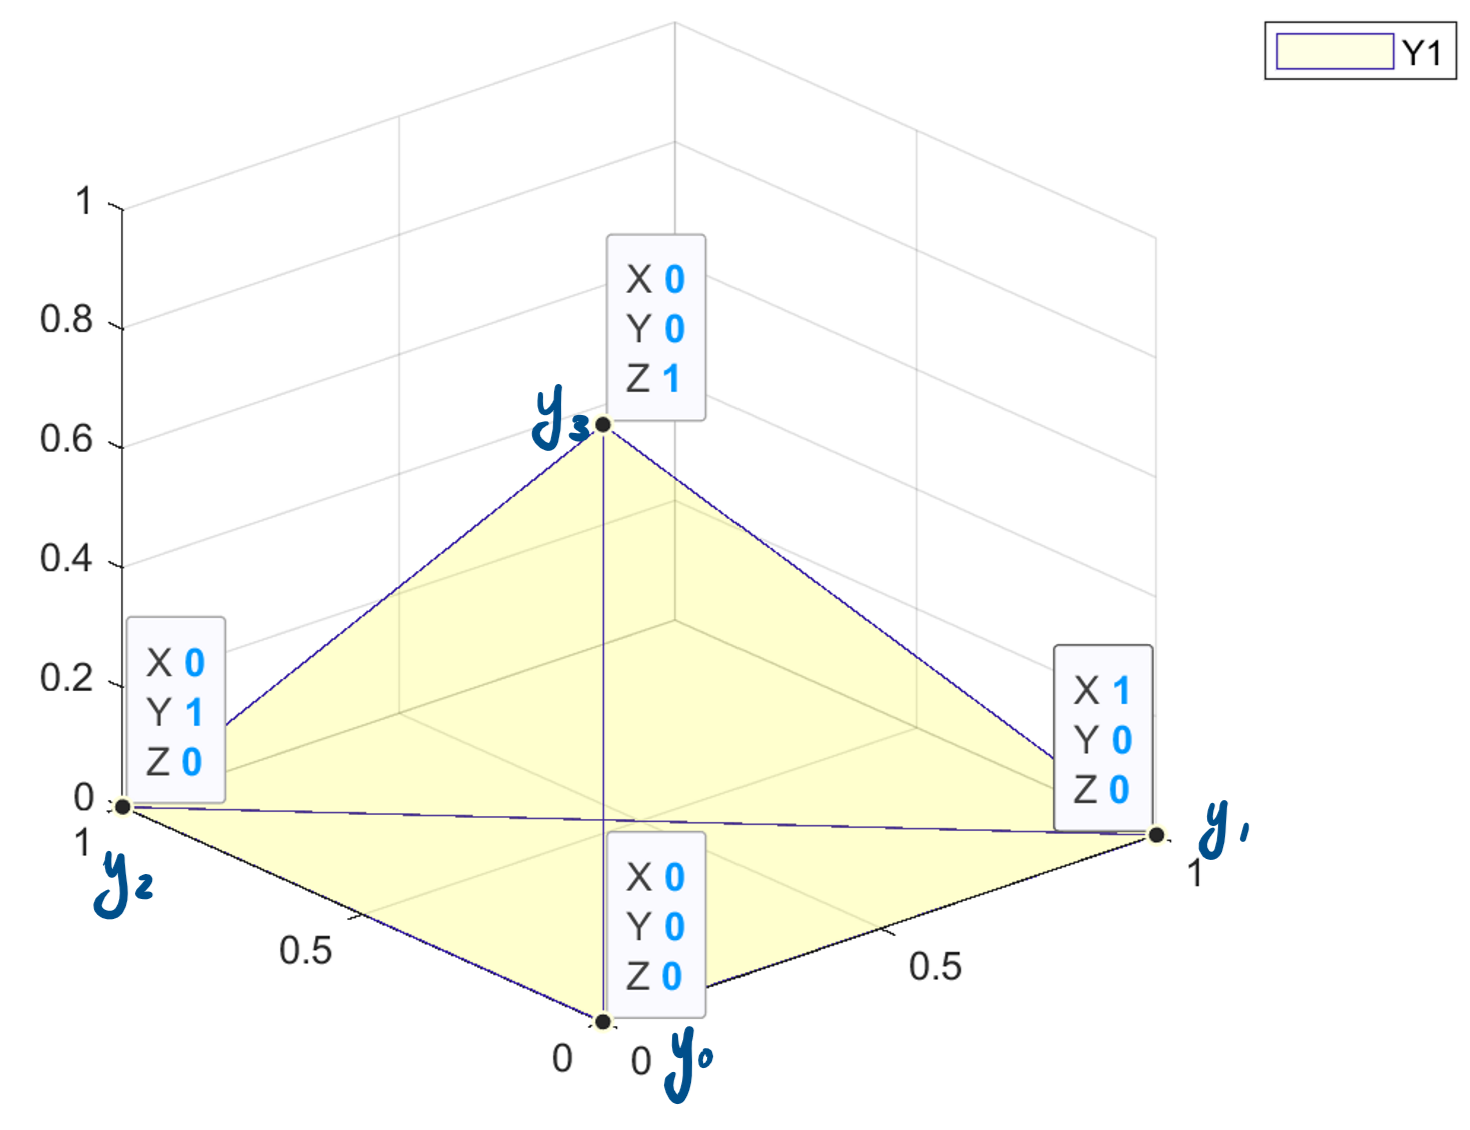
\includegraphics[width=0.45\linewidth]{InitializeFig}
\end{frame}

\begin{frame}{1. Order, create centroid, and compute $x^r$}
	\centering
	\includegraphics[width=0.45\linewidth]{Order}
	\includegraphics[width=0.45\linewidth]{OrderFig}
\end{frame}

\begin{frame}{2. Reflect}
	\centering
	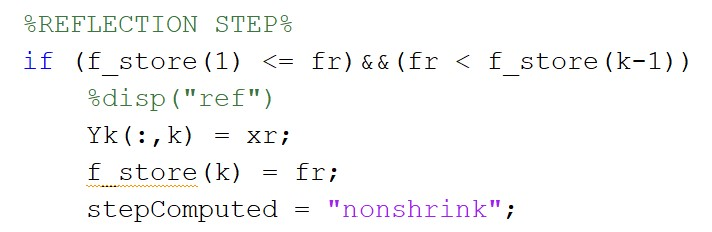
\includegraphics[width=0.45\linewidth]{Reflect}
	\includegraphics[width=0.45\linewidth]{RefelctFig}
\end{frame}

\begin{frame}{3. Expand}
	\centering
	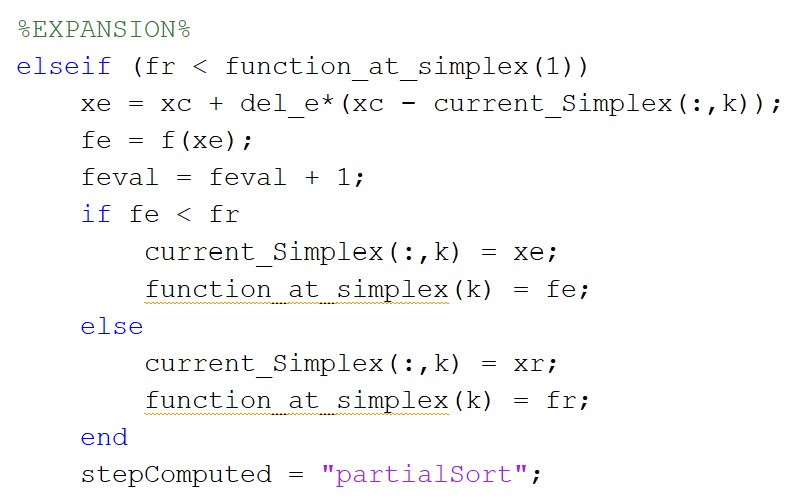
\includegraphics[width=0.45\linewidth]{Expand}
	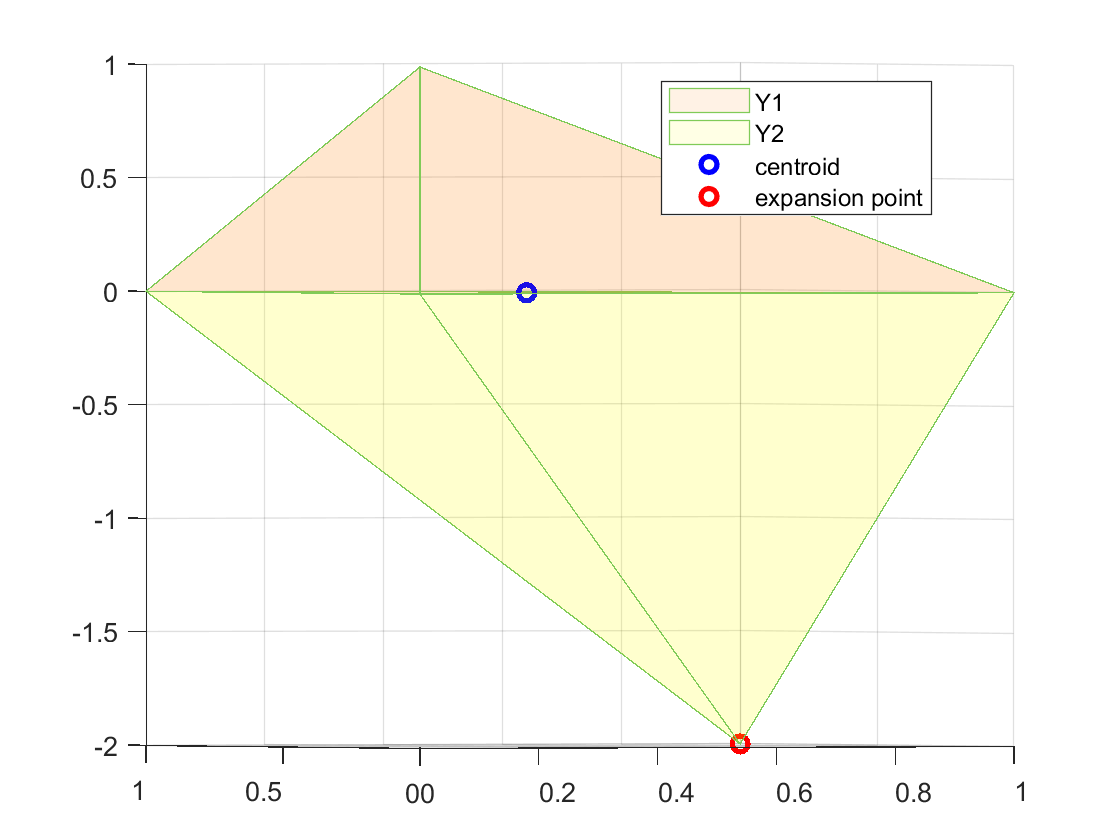
\includegraphics[width=0.45\linewidth]{ExpandFig}
\end{frame}

\begin{frame}{4.a) Outside Contraction}
	\centering
	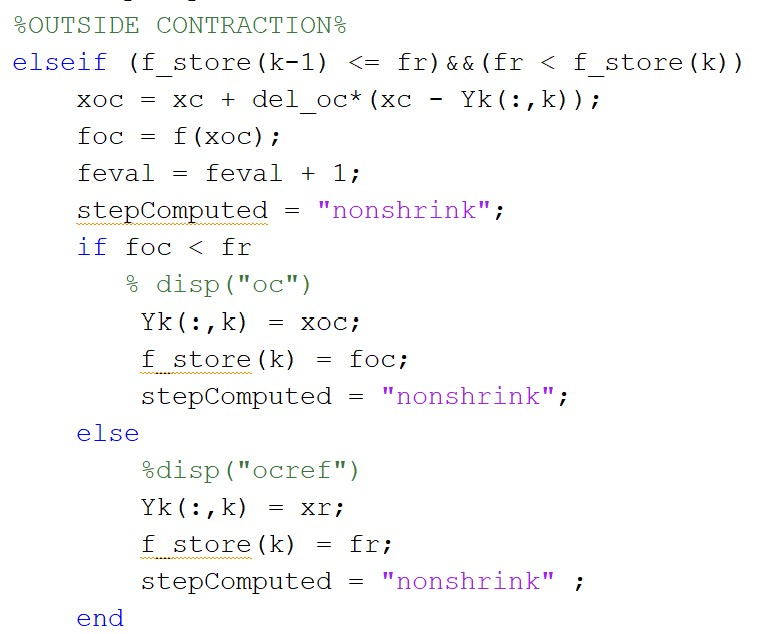
\includegraphics[width=0.45\linewidth]{OC}
	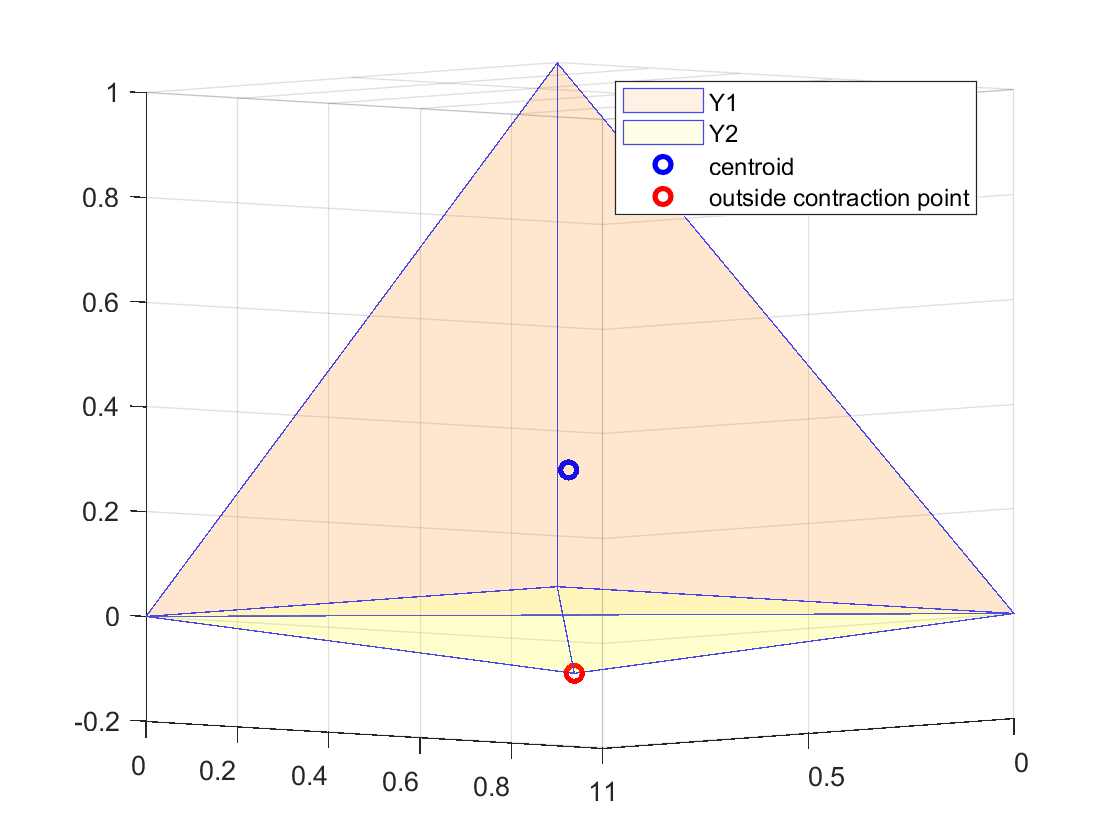
\includegraphics[width=0.45\linewidth]{OCFig}
\end{frame}

\begin{frame}{4.b) Inside Contraction}
	\centering
	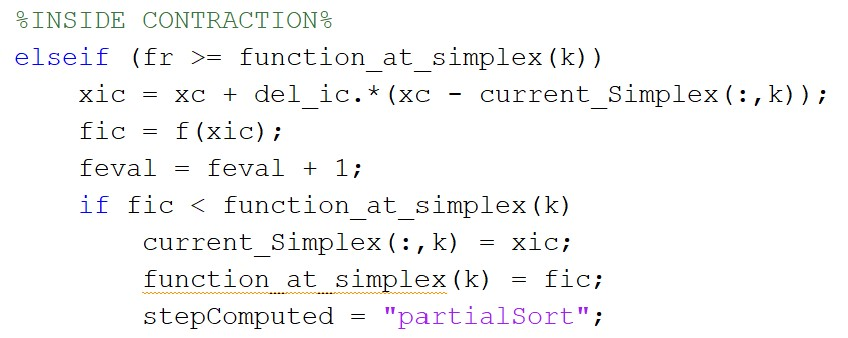
\includegraphics[width=0.45\linewidth]{IC}
	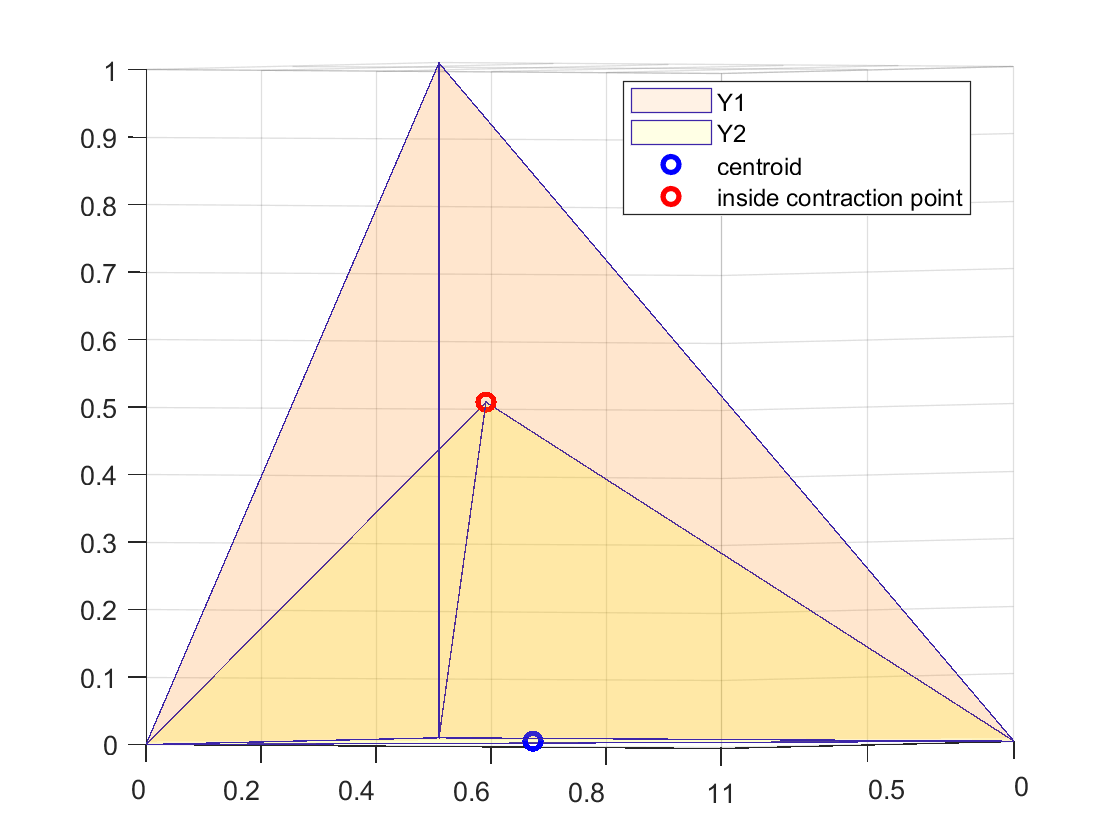
\includegraphics[width=0.45\linewidth]{ICFig}
\end{frame}

\begin{frame}{5. Shrink}
	\centering
	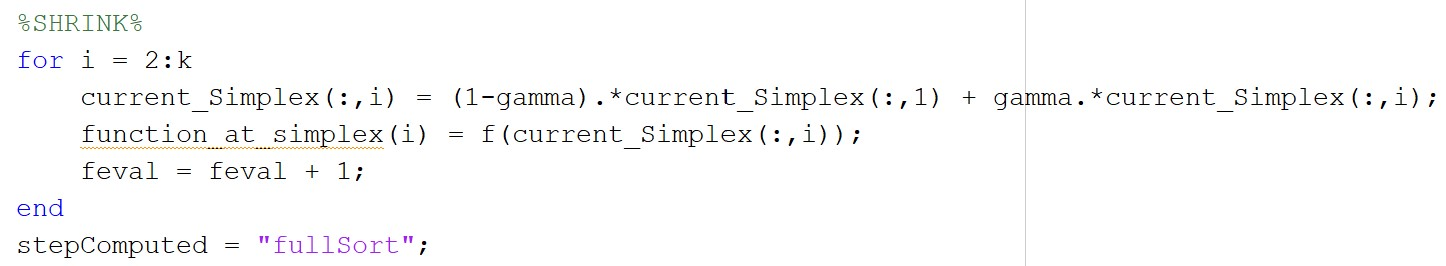
\includegraphics[width=0.45\linewidth]{Shrink}
	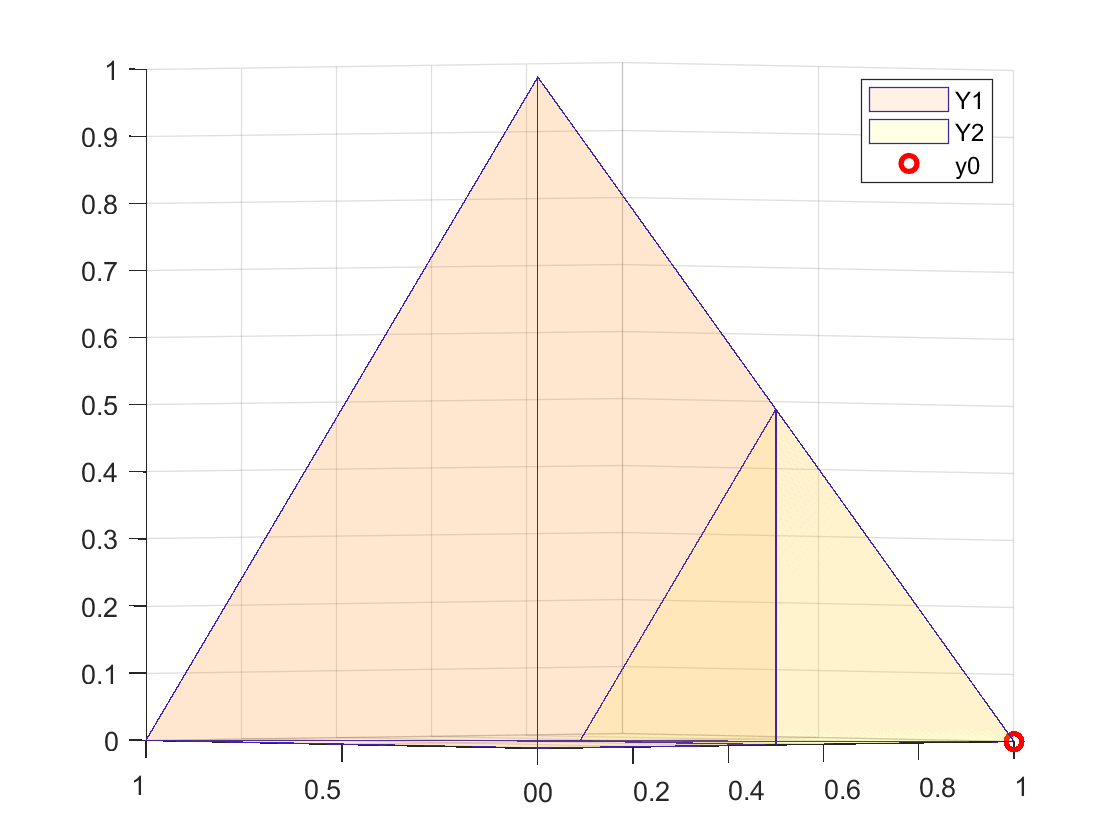
\includegraphics[width=0.45\linewidth]{ShrinkFig}
\end{frame}

\end{document}